\documentclass[a4paper]{jpconf}
\usepackage{graphicx}
%\usepackage{draftwatermark}
\usepackage[margin=0.7in]{geometry}
\usepackage{lmodern}% http://ctan.org/pkg/lm
\usepackage{listings}
\usepackage{pgfplots}
\usepackage{wrapfig}
\usepackage{multicol}
\usepackage[utf8]{inputenc}
\usepackage[toc,page]{appendix}
%\usepackage{wrapfig}
%\usepackage{float}
\usepackage{hyperref}
\usepackage{listings}
\usepackage{changepage}
\usepackage{caption}
\usepackage{color}
\usepackage{beramono}
\usepackage{xcolor}
\usepackage{courier}
\usepackage{subcaption}
\usepackage{hyperref}\begin{document}
\title{Profiling CPU-bound workloads on Intel Haswell-EP platforms}

\author{M Guerri$^1$, D Giordano$^1$ and C Cordeiro$^1$}
\address{$^1$ CERN}
\ead{marco.guerri@cern.ch}
%\SetWatermarkText{DRAFT}
\definecolor{lightblue}{gray}{0.96}

\lstset{
    language=Python,
    basicstyle=\ttfamily\scriptsize,
    tabsize=2,
    backgroundcolor=\color{lightblue},
    captionpos=b,
    columns=fixed,
    numbers=left,
    columns=fullflexible,
    keepspaces=true,
    showstringspaces=false,
    stepnumber=1,
    numberstyle=\zebra{lightblue}{white},
    numbersep=5pt,
    frame=lines,
    escapeinside={£}{£},
    postbreak=\raisebox{0ex}[0ex][0ex]{\ensuremath{\color{red}\hookrightarrow\space}},
    breaklines=true,
    keywordstyle=\color[rgb]{0,0,1},
    commentstyle=\color[rgb]{0.133,0.545,0.133},
    stringstyle=\color[rgb]{1,0,0}
}

\lstdefinelanguage
   [x64]{Assembler}
   [x86masm]{Assembler}
   {morekeywords={CDQE,CQO, CMPB, CMPSQ,CMPXCHG16B,JRCXZ,LODSQ,MOVSXD,
                  POPFQ,PUSHFQ,SCASQ,STOSQ,IRETQ,RDTSCP,SWAPGS,MOVL,VMOVAPD,
                  VSTMXCSR, VMOVSD, MOVABS, MOVQ, ADDSD, MOVAPD, MULSD, NOPL,
                  rax,rdx,rcx,rbx,rsi,rdi,rsp,rbp, rip,
                  r8,r8d,r8w,r8b,r9,r9d,r9w,r9b, r12, r13, r14, r15,
                  xmm0, xmm1, xmm2, xmm3},
    deletekeywords=[2]{code}
    }
\newcommand\realnumberstyle[1]{}

\makeatletter
\newcommand{\zebra}[3]{%
    {\realnumberstyle{#3}}%
    \begingroup
    \lst@basicstyle
    \ifodd\value{lstnumber}%
        \color{#1}%
    \else
        \color{#2}%
    \fi
        \rlap{\hspace*{\lst@numbersep}%
        \color@block{\linewidth}{\ht\strutbox}{\dp\strutbox}%
        }%
    \endgroup
}
\makeatother


\begin{abstract}
With the increasing adoption of cloud resources, public and private, to support
the demands in terms of computing capacity of the WLCG, the HEP community has begun
studying several benchmarking applications aimed at continuously assessing the
performance of virtual machines procured from commercial providers.
In order to characterise the behaviour of these benchmarks, in-depth
profiling activities have been carried out. In this document we outline
our experience in profiling one specific application, ATLAS Kit Validation,
in an attempt to explain an unexpected distribution of the performance samples
obtained on systems based on Intel Haswell-EP processors.
\end{abstract}


\section{Introduction}
Nowadays the majority of the experiments' workloads running on the WLCG are simulation 
jobs, where most of the computing time is spent in CPU-bound activities. For this 
reason the adoption of fast benchmarks representative of these workloads 
can be beneficial for monitoring and resource allocation purposes,
by providing real-time information on the performance delivered by virtual 
machines in the cloud or job slots in a grid site.
%For instance a prompt benchmarking can  act as a prediction mechanism for the 
%execution of the LHC experiments' workloads, allowing for a fast and reliable 
%triage of suitable resources in a much shorter time period than standard jobs.
A number of fast benchmarks is being studied by the HEP community. Within the 
HEPiX Benchmarking Working Group~\cite{HEPiX:2014:HEPiX}, two fast benchmarks are 
in particular under deep investigation: Dirac Benchmark 2012 (DB12)~\cite{CERN:2016:DB12} 
and ATLAS Kit Validation (KV)~\cite{KV}.

\section{KV Benchmark}
KV is the toolkit adopted by the ATLAS collaboration for the
validation of their software installation in grid sites. The tests include, among
others, the GEANT4~\cite{GEANT4} simulation of the ATLAS detector, which
has been re-purposed to benchmark compute resources against CPU-bound 
workloads. The KV benchmark simulates $n$ independent events consisting of a single muon particle 
propagating through the ATLAS detector. The CPU time needed to elaborate each event 
is recorded and the average over the $n$ events is computed as the final benchmark result.
By excluding the first event in the sequence from the final average, spurious effects such as the 
overhead coming from the initialisation of the software libraries and the configuration 
of the simulation parameters (detector geometry, list of particles, properties of 
the materials) are disregarded from the measurement.

The KV benchmark is single threaded as most of the LHC experiments'
software applications. In order to fully utilize compute resources and reproduce
the worst case load scenario, where all compute slots are running jobs and
CPU idle time is minimised, the benchmark is configured to run,
by default, in parallel with as many threads as the number of logical cores 
provided by the server and the benchmark result is calculated as the arithmetic 
average over all threads.

In the past few years the KV benchmark has been used to assess the performance of
resources provided by commercial cloud providers and grid site. The results 
have been compared with the average CPU time required to simulate ATLAS events, 
as reported by the experiment's job monitoring framework. Details about this activity 
and the correlation among benchmark results and job duration are reported 
in~\cite{bmk}.


\section{Investigating KV results}
One of the several environments that was benchmarked using KV consisted of
 240 Haswell-EP hypervisors providing compute
resources as VMs dedicated to the CERN Tier-0 batch system. The servers were
fitted with two 8-core Intel Xeon E5-2630v3 processors, with a total number  
of 32 threads per server with simultaneous multithreading enabled, and 64~GiB    
of DDR4 RAM in fully balanced configuration, with each memory channel populated with
the same number of DIMMs of equal capacity. All the hypervisors were configured 
to host 2 VMs providing 16 virtual processing units each, with pairs of VMs 
confined to separate NUMA domains. KV was executed with 16 parallel processes 
on each VM, resulting in the full utilisation of the hardware threads provided
by the machine, and the final aggregated result was obtained as the average over 
the 16 simulation times. The samples collected from the VMs under test resulted in a dual-mode guassian distribution, with a 2\% difference between the 
mean of the two modes as shown in Figure~\ref{dual-mode-gaussian}.


\begin{figure}[ht]
\begin{center}
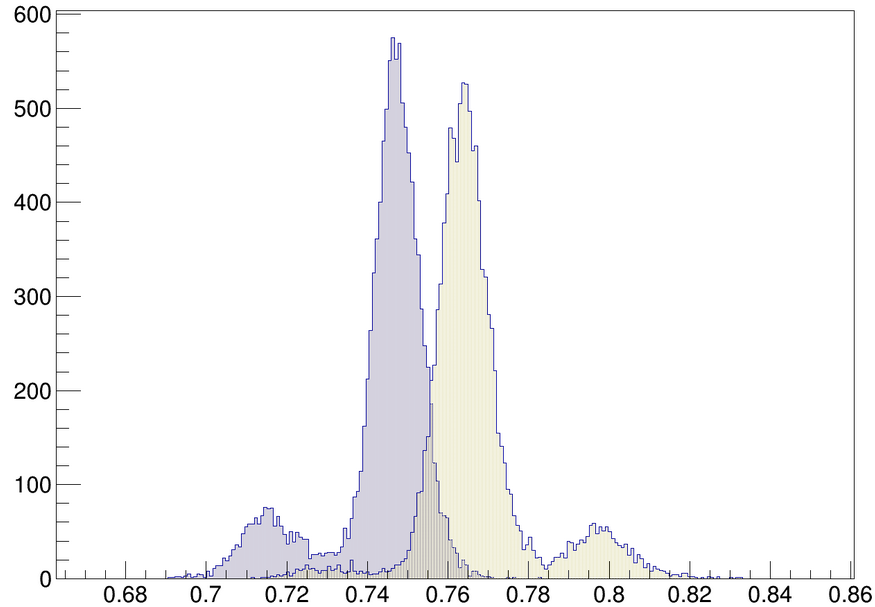
\includegraphics[width=0.5\textwidth]{images/dual-mode-gaussian.png}
\end{center}
\caption{\label{dual-mode-gaussian} Distribution of the average KV execution speed [sec/evt] on  VMs with 16 virtual CPUs. }
\end{figure}




%\section{Bare metal results}
In order to ease the performance analysis, the virtualisation layer was
temporarily removed and simultaneous multithreading disabled, running KV on
the bare-metal server installed with CentOS 7 while setting scheduling affinity sequentially to each physical
core. The results shown in table ~\ref{table:simulation-time-cores}
highlighted a 12\% difference in the average simulation
time when binding KV to core 8, the first core of the second processor (CPU1).

%\begin{figure}[h]
%\begin{center}
%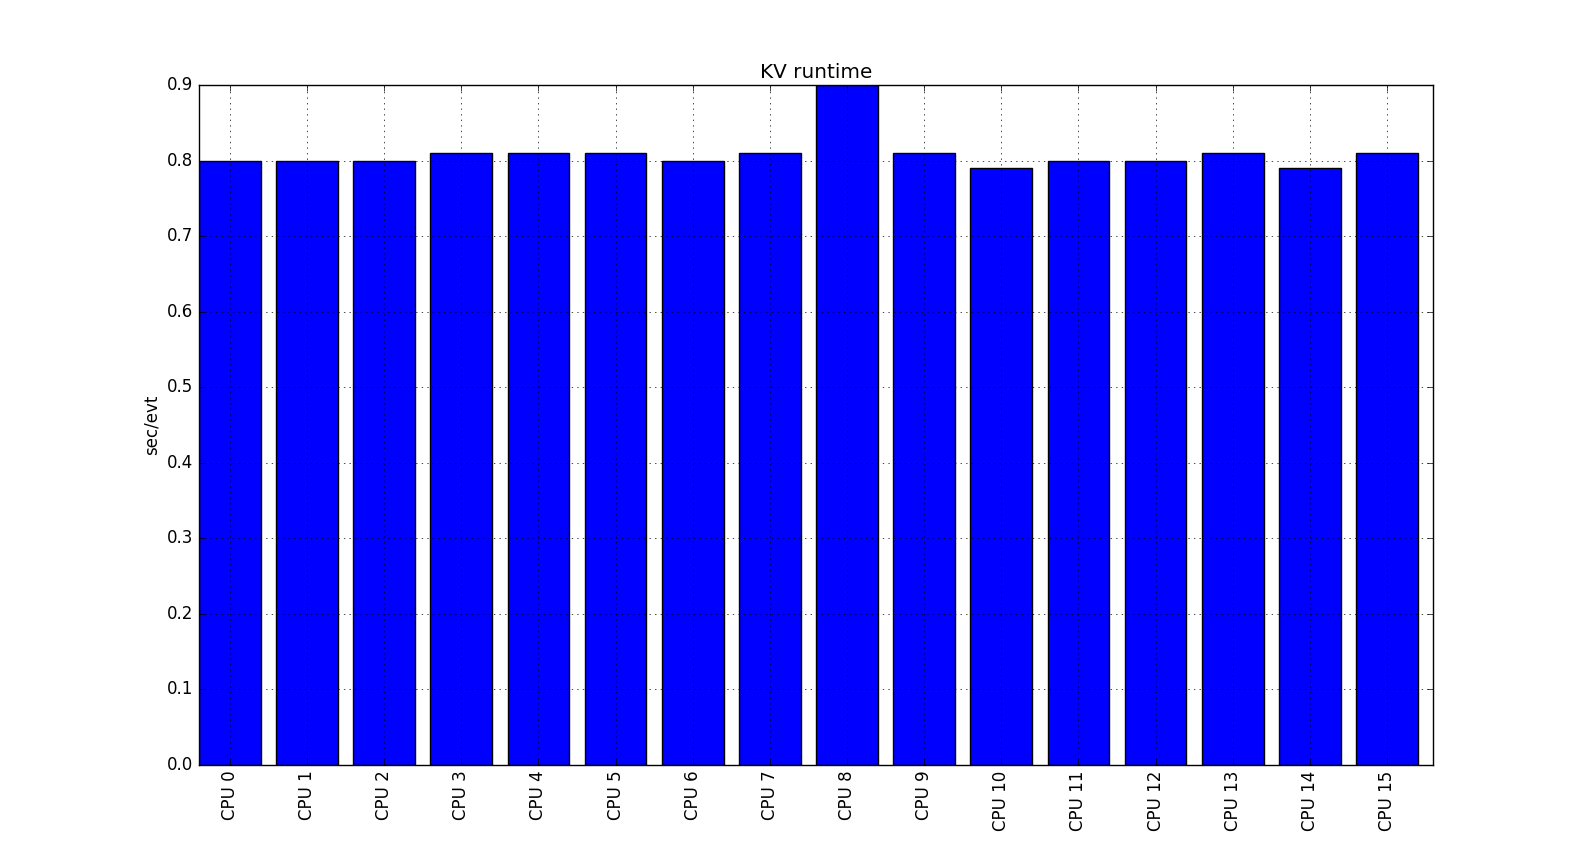
\includegraphics[scale=0.3]{images/kv_runtime.png}
%\end{center}
%\caption{\label{kv-runtime} Bare-metal KV performance (sec/evt) on each physical core. }
%\end{figure}

\begin{wraptable}{l}{0.35\linewidth}
    \vspace{-3mm}
    \caption{Average simulation time \newline (sec/evt) on bare-metal server \newline 
             running CentOS 7}
    \label{table:simulation-time-cores}
    \begin{tabular}{ |l |  l  || l | l|}
        \hline
        \multicolumn{2}{|c||}{CPU0} & \multicolumn{2}{|c|}{CPU1} \\
        \hline
         Core 0  & 0.80 & Core 8  & 0.90\\
        \hline
         Core 1  & 0.80 & Core 9  & 0.81\\
        \hline
         Core 2  & 0.80 & Core 10  & 0.79\\
        \hline
         Core 3  & 0.81 & Core 11  & 0.80\\
        \hline
         Core 4  & 0.81 & Core 12  & 0.80\\
        \hline
         Core 5  & 0.81 & Core 13  & 0.81\\
        \hline
         Core 6  & 0.80 & Core 14 & 0.79\\
        \hline
        Core 7  & 0.81 & Core 15  & 0.81\\
        \hline
    \end{tabular}
    \vspace{-7mm}
\end{wraptable}
Further tests confirmed the same behaviour also with simultaneous multithreading
enabled, with slower performance on threads 8 and 24, both belonging to the first core of
CPU1. Single-threaded runs in a virtualised environment showed a 16\%
increase in the final average simulation time when running on virtual processors
corresponding to hardware threads 8 and 24, confirming the 2\%
spread that stood out from the statistical distribution after averaging the results
over all 8 virtual processors within each VM. This performance discrepancy
was not observed with any other benchmark under study within the HEPiX Benchmarking
Working Group.


\section{Profiling single events}
A deeper dive in the logs showed that all the events required more time to be
simulated on core 8. In particular, event 73 was identified as the one
requiring the longest simulation time: ~34 seconds on core 8 against ~29 seconds
on any other core, making it a good candidate for a detailed analysis. Profiling
a single event required a way to attach \textit{perf} to KV only during the time frame
where one specific simulation was being executed. The solution adopted consisted
of a Python script which would monitor KV log files via \textit{pyinotify} to detect
the beginning of event 73 and then attach \textit{perf} to the process until the
detection of the end of the event. One essential requirement for this to work correctly
was to disable all the buffering carried out at any layer of the stack before
data actually reached the storage device. KV writes log files via Python code,
therefore the following points had to be taken into consideration:
%\begin{lstlisting}[caption=Simulation of event 73 on core 8, basicstyle=\scriptsize]
%*  Memory snooper called at end of event with VMEM: 1443232kB
%G4SimTimer           INFO        Event nr. 73 took 34.58 s. New average 0.985 +- 0.4806
%AtRndmGenSvc         INFO  Stream =  SINGLE, Seed1 =  93448506, Seed2 = 144728191
%AthenaEventLoopMgr   INFO  done processing event #72, run #1 73 events processed so far
%AthenaEventLoopMgr   INFO  start processing event #73, run #1 73 events processed so far
%G4AtlasAlg           INFO ++++++++++++  G4AtlasAlg execute  ++++++++++++
%\end{lstlisting}

%\begin{lstlisting}[caption=Simulation of event 73 on core 0, basicstyle=\scriptsize]
%*  Memory snooper called at end of event with VMEM: 1443252kB
%G4SimTimer           INFO        Event nr. 73 took 29.68 s. New average 0.8681 +- 0.4133
%AtRndmGenSvc         INFO  Stream =  SINGLE, Seed1 =  93448506, Seed2 = 144728191
%AthenaEventLoopMgr   INFO  done processing event #72, run #1 73 events processed so far
%AthenaEventLoopMgr   INFO  start processing event #73, run #1 73 events processed so far
%G4AtlasAlg           INFO ++++++++++++  G4AtlasAlg execute  ++++++++++++
%\end{lstlisting}

\begin{itemize}
\item A call to the \textit{open} function in Python results in the invocation
of libc \textit{fopen}. Python can modify libc buffering behaviour via the libc
function \textit{setvbuf} if \textit{buffering} parameter is specified,
otherwise the default buffering mode is used.
\item The environment variable \textit{PYTHONUNBUFFERED} can be used to turn off
buffering of \textit{stdin, stdout and stderr}.
\end{itemize}
Without control over the Python source code, unbuffered I/O was implemented by 
invoking KV with \textit{stdbuf -o0} command and redirecting \textit{stdout} and \textit{stderr}
to an additional file that would be monitored by the \textit{pyinotify} script. This approach 
works correctly even when commands are piped together.
\\
The profile of the execution was obtained with \textit{perf record}.
Results for core 0
and core 8 are shown respectively in Listing~\ref{event-73-processor0} and
Listing~\ref{event-73-processor8}, limiting the output to functions that
contribute for more than 1\% of the runtime.

\begin{lstlisting}[caption=Recording of event 73 on core 0., label=event-73-processor0]
# Samples: 125K of event ' cycles:pp'
# Event count (approx.): 99035639955
#
# Overhead  Command    Shared Object          Symbol
#
    12.72%  athena.py  libm-2.17.so           [.] __ieee754_log_avx
     7.36%  athena.py  libm-2.17.so           [.] __ieee754_exp_avx
     5.51%  athena.py  libG4global.so         [.] G4PhysicsVector::Value
     3.64%  athena.py  libG4processes.so      [.] G4UniversalFluctuation::SampleFluctuations
     3.25%  athena.py  libm-2.17.so           [.] __GI___exp
     2.67%  athena.py  libm-2.17.so           [.] __sin_avx
     2.54%  athena.py  libMagFieldServices.so [.] BFieldCache::getB
     2.26%  athena.py  libG4tracking.so       [.] G4SteppingManager::DefinePhysicalStepLength
     2.13%  athena.py  libm-2.17.so           [.] __cos_avx
     1.81%  athena.py  libG4geometry.so       [.] G4Navigator::LocateGlobalPointWithinVolume
     1.69%  athena.py  libG4tracking.so       [.] G4SteppingManager::InvokePSDIP
     1.62%  athena.py  libm-2.17.so           [.] __log10_finite
     1.46%  athena.py  libm-2.17.so           [.] __sincos
     1.45%  athena.py  libG4geometry.so       [.] G4PropagatorInField::ComputeStep
     1.28%  athena.py  libG4processes.so      [.] G4UrbanMscModel93::SampleCosineTheta
     1.26%  athena.py  libG4tracking.so       [.] G4SteppingManager::Stepping
     1.17%  athena.py  libG4geometry.so       [.] G4AtlasRK4::Stepper
     1.14%  athena.py  libG4processes.so      [.] G4VEnergyLossProcess::PostStepGetPhysicalInter
     1.06%  athena.py  libG4processes.so      [.] G4ElectroNuclearCrossSection::GetZandACrossSec
\end{lstlisting}

\begin{lstlisting}[caption=Recording of event 73 on core 8., label=event-73-processor8]
# Samples: 141K of event ' cycles:pp'
# Event count (approx.): 111860905419
#
# Overhead  Command    Shared Object                      Symbol
#
    11.38%  athena.py  libm-2.17.so           [.] __ieee754_log_avx
     6.44%  athena.py  libm-2.17.so           [.] __ieee754_exp_avx
     4.90%  athena.py  libG4global.so         [.] G4PhysicsVector::Value
     3.38%  athena.py  libG4processes.so      [.] G4UniversalFluctuation::SampleFluctuations
     2.88%  athena.py  libm-2.17.so           [.] __GI___exp
     2.64%  athena.py  libm-2.17.so           [.] __sin_avx
     2.51%  athena.py  libMagFieldServices.so [.] BFieldCache::getB
     1.93%  athena.py  libG4tracking.so       [.] G4SteppingManager::DefinePhysicalStepLength
     1.83%  athena.py  libm-2.17.so           [.] __cos_avx
     1.78%  athena.py  libG4geometry.so       [.] G4Navigator::LocateGlobalPointWithinVolume
     1.59%  athena.py  libm-2.17.so           [.] __log10_finite
     1.45%  athena.py  libG4tracking.so       [.] G4SteppingManager::InvokePSDIP
     1.37%  athena.py  libG4geometry.so       [.] G4PropagatorInField::ComputeStep
     1.36%  athena.py  libm-2.17.so           [.] __sincos
     1.28%  athena.py  libG4processes.so      [.] G4VEnergyLossProcess::PostStepGetPhysicalInteractionLength
     1.18%  athena.py  libG4tracking.so       [.] G4SteppingManager::Stepping
     1.15%  athena.py  libG4processes.so      [.] G4UrbanMscModel93::SampleCosineTheta
     1.01%  athena.py  libG4tracking.so       [.] G4SteppingManager::InvokeAlongStepDoItProcs
     1.01%  athena.py  libG4geometry.so       [.] G4AtlasRK4::Stepper

\end{lstlisting}
%\begin{figure}[h]
%\begin{center}
%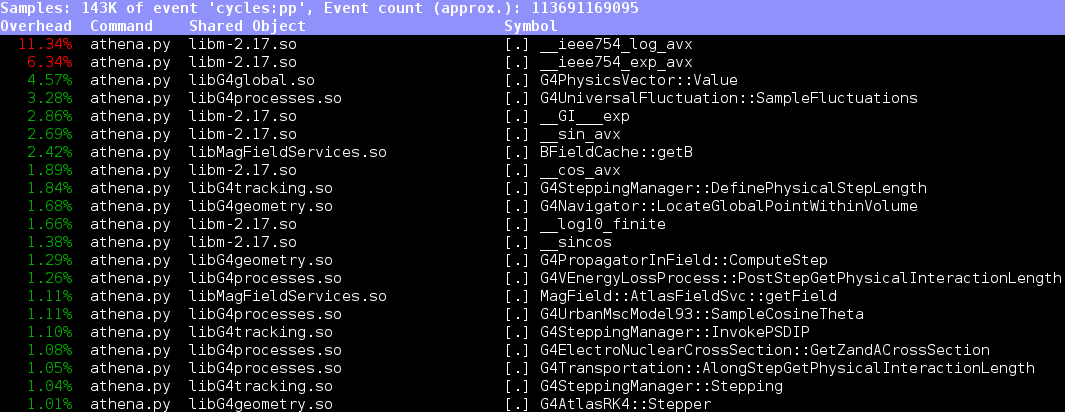
\includegraphics[scale=0.45]{images/Event73_Processor8.png}
%\end{center}
%\caption{\label{event-73-processor8} Recording of event 73 on core 8}
%\end{figure}

%\begin{figure}[h]
%\begin{center}
%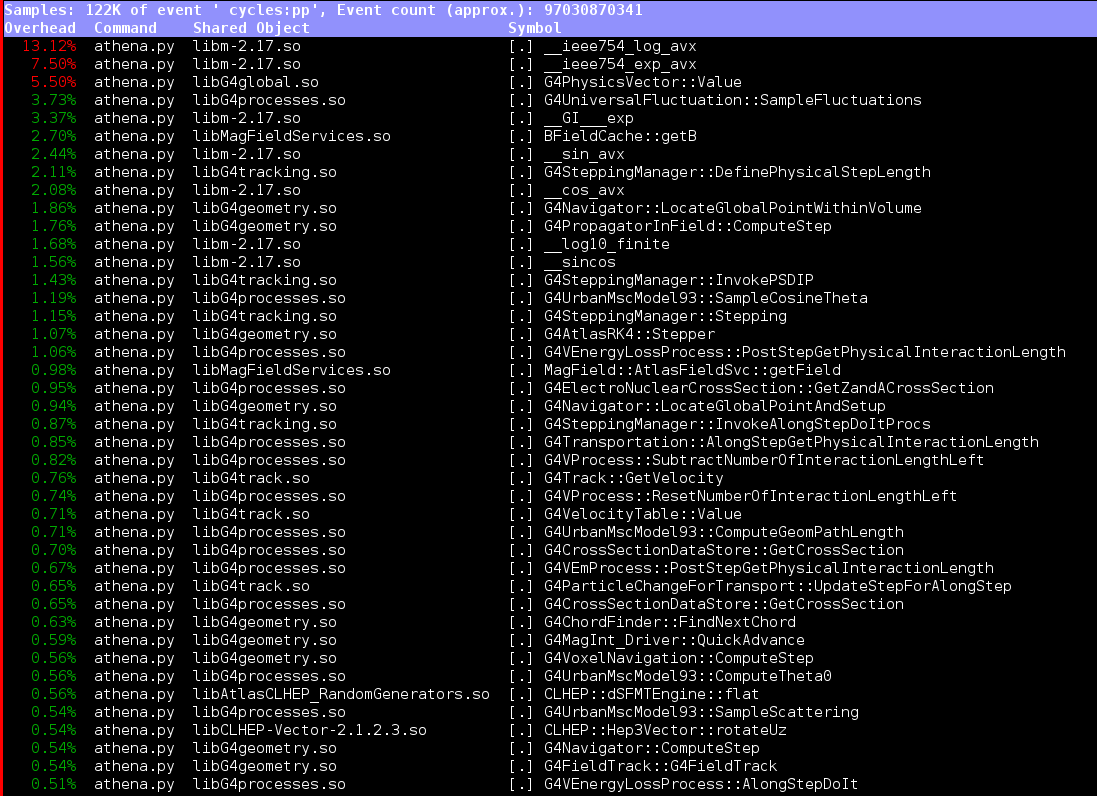
\includegraphics[scale=0.45]{images/Event73_Processor0.png}
%\end{center}
%\caption{\label{event-73-processor0} Recording of event 73 on core 0}
%\end{figure}

Excluding the higher number of events (unhalted core cycles) on core 8, which was 
expected due to the longer runtime, it was not possible to identify any major differences 
between the two runs. A list of the top contributors to the additional clock cycles required 
when running on core 8 was extracted from the recordings. Results are shown in Table~\ref{major-contributors}.

\begin{table}[ht]
\begin{center}
\begin{tabular}{ | l | l |}
  \hline
  G4StepLimiter::PostStepGetPhysicalInteractionLength &  2.67\% \\
  \hline
  \_\_sin\_avx & 2.45\% \\
  \hline
  G4VEnergyLossProcess::PostStepGetPhysicalInteractionLength & 2.37\% \\
  \hline
  FADS::FadsSteppingAction::UserSteppingAction & 2.33\% \\
  \hline
  \_ZN12G4FieldTrackC1ERKN5CLHEP10Hep3VectorES3\_ddddddPS2\_@plt & 2.27\% \\
  \hline
  BFieldCache::getB & 2.22\% \\
  \hline
  \_ZN11TrackHelperC1EPK7G4Track@plt & 2.08\% \\
  \hline
  G4CrossSectionDataStore::GetCrossSection & 2.06\% \\
  \hline
  G4SteppingManager::InvokeAlongStepDoItProcs & 2.01\% \\
  \hline
  G4Transportation::AlongStepGetPhysicalInteractionLength & 1.85\% \\
  \hline
  G4FieldTrack::G4FieldTrack & 1.69\% \\
  \hline
  std::\_Rb\_tree\_increment & 1.66\% \\
  \hline
  G4Mag\_EqRhs::SetChargeMomentumMass & 1.63\% \\
  \hline
  G4Navigator::LocateGlobalPointWithinVolume & 1.56\% \\
  \hline
  G4ParticleChangeForTransport::UpdateStepForAlongStep & 1.43\% \\
  \hline
  \_\_log10\_finite & 1.39\% \\
  \hline
\end{tabular}
\end{center}
\caption{Major contributors to the additional runtime on core 8 (percentage
of the additional clock cycles) }
\label{major-contributors}
\end{table}

\section{Profiling the major contributors}
The functions appearing in Table~\ref{major-contributors} were profiled to obtain
a detailed breakdown of the weight of each assembly instruction in terms of
clock cycles. The most relevant recordings are reported in Appendix~\ref{appendix:function-recordings}. 
The results highlighted an interesting pattern on most of the major contributors to 
the additional runtime on core 8:  it appeared that an unexpectedly
large number of cycles was attributed to the initial instructions of each function,
most of which could not justify such a high cost. In some cases a
\textit{mov} of a literal value to a register was taking up 8\% of the whole
execution time of that specific function (Listing~\ref{lst:log10}).
Such behaviour was common to all cores and could not explain the performance
asymmetry highlighted by the benchmark, but it was reasonable to hypothesize
a correlation with this peculiar profile. A first hypothesis
pointed in the direction of instruction cache misses as the reason behind
the overhead attributed to the initial instructions.
ATLAS Kit Validation seemed a good candidate for a large number of such events,
with its code segment consisting of more than 300 shared libraries.

\section{A synthetic benchmark to generate instruction cache misses}
A synthetic benchmark aimed at causing a large number of instruction cache
misses was automatically generated using a \href{https://gitlab.cern.ch/snippets/216}{Python script} ~\cite{synthetic_benchmark:icache_misses}.
The resulting C code was compiled
under CentOS 7 with gcc 4.8.5 and optimizations disabled (\textit{-O0}). The benchmark 
consists of a large number of dummy functions which are called randomly at runtime to generate
repeated instruction cache misses in L1i and L2. Interestingly, the results
highlighted the same performance asymmetry observed with ATLAS Kit Validation,
with a 20\% increase in runtime on core 8 with respect to the other cores.
This effect could only be observed on Haswell-EP, Haswell-EX (quad-socket, with
a single core on two different sockets affected) and Broadwell-EP systems. It
was not possible to reproduce a similar performance asymmetry on Sandy Bridge
and Ivy Bridge platforms.
%\begin{figure}[h]
%\begin{center}
%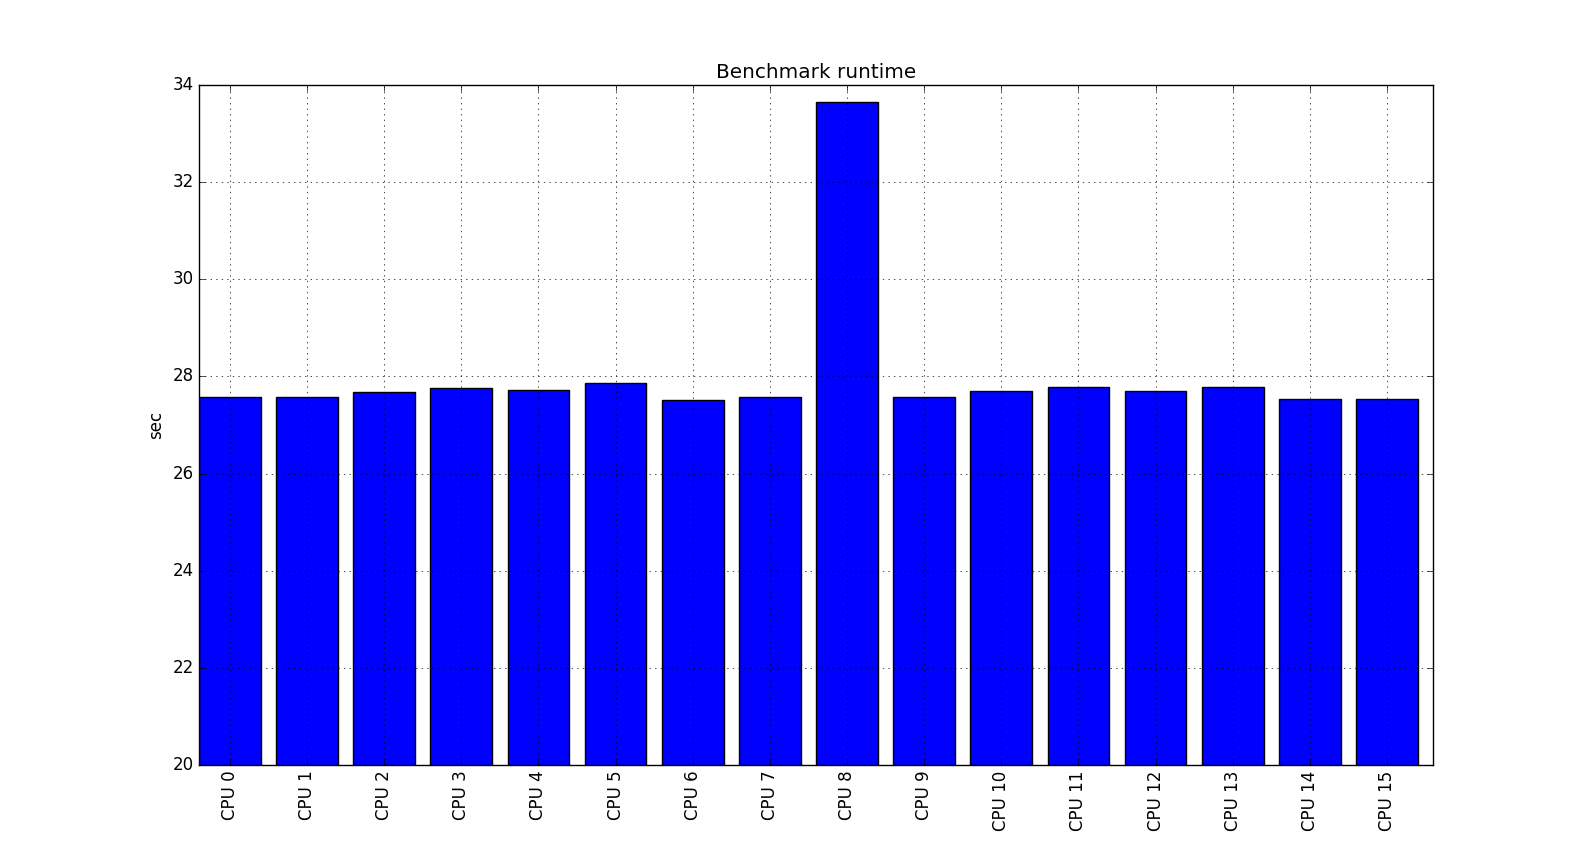
\includegraphics[scale=0.45]{images/syn-bench-a.png}
%\end{center}
%\caption{\label{syn-bench-a} Runtime of the synthetic benchmark (random calls)}
%\end{figure}
Further investigations succeeded in generating
workloads with similar relative number of L1i and L2 instruction cache misses
on Haswell and Broadwell, but without any discrepancy in execution time,
disproving the initial hypothesis and making it necessary to seek for an
alternative explanation.

\section{An additional benchmark with customizable code segment size}
\label{section:benchmark-itlb}
\href{https://gitlab.cern.ch/snippets/217}{A second synthetic benchmark}
was written in order to verify the existence of a
correlation between the size of the code segment and the slowdown observed on core 8
~\cite{synthetic_benchmark:icache_misses_variable_code_segment}. 
This benchmark also aims to generate instruction cache misses,
but within a code segment whose size can be controlled via a command line
argument. The code makes use of a large switch statement that dispatches
randomly generated opcodes in loop. By feeding the switch with \textit{opcode mod n}, the number of case
branches effectively used at runtime is limited to $n$. The higher $n$, the larger the
number of case branches that can be reached. By sampling the
maximum and minimum values of \textit{rip} register, a reliable estimate of the
size of the hot portion of the code segment is obtained. The
benchmark takes $n$ as command line argument and prints a tuple consisting of
three values: \textit{size code segment, runtime without initialization} and \textit{n}.
The graph in Figure~\ref{fig:runtime-difference} shows the difference in runtime
between core 8 and core 0 with respect to the size of the code segment. After having
filtered out a negligible number of outliers (1.5\% of the measurements),
the samples collected clearly highlighted a performance
degradation beyond approximately 512KiB, with core 8 running up to 4 seconds slower
(9.4\%) in the 3MB area. 512KiB is an interesting number, as it
corresponds to the space addressable with 128 iTLB entries using 4KiB pages: this
matches exacly the size of the iTLB on Haswell and Broadwell architectures.
With a code segment larger than 512KiB, a heavily nonlinear execution flow starts generating an increasingly
large number of iTLB misses and a diverging performance possibly points in the direction of different
behaviour of the pipeline front-end in handling such events. The test was repeated 
by making use of the huge pages support of the operating
system (2MiB) to map the code segment of the benchmark. With this setup no 
performance difference was observed between core 8 and the other cores on the system.
%\begin{lstlisting}[caption=Compilation and execution of the synthetic benchmark using huge pages]
%sysctl vm.nr_hugepages=500
%gcc benchmark.c -o benchmark -O0 -B/usr/share/libhugetlbfs -Wl,--hugetlbfs-align
%hugectl --text ./switch_slowdown_v2 32768
%\end{lstlisting}

%\begin{figure}[ht]
%\begin{center}
%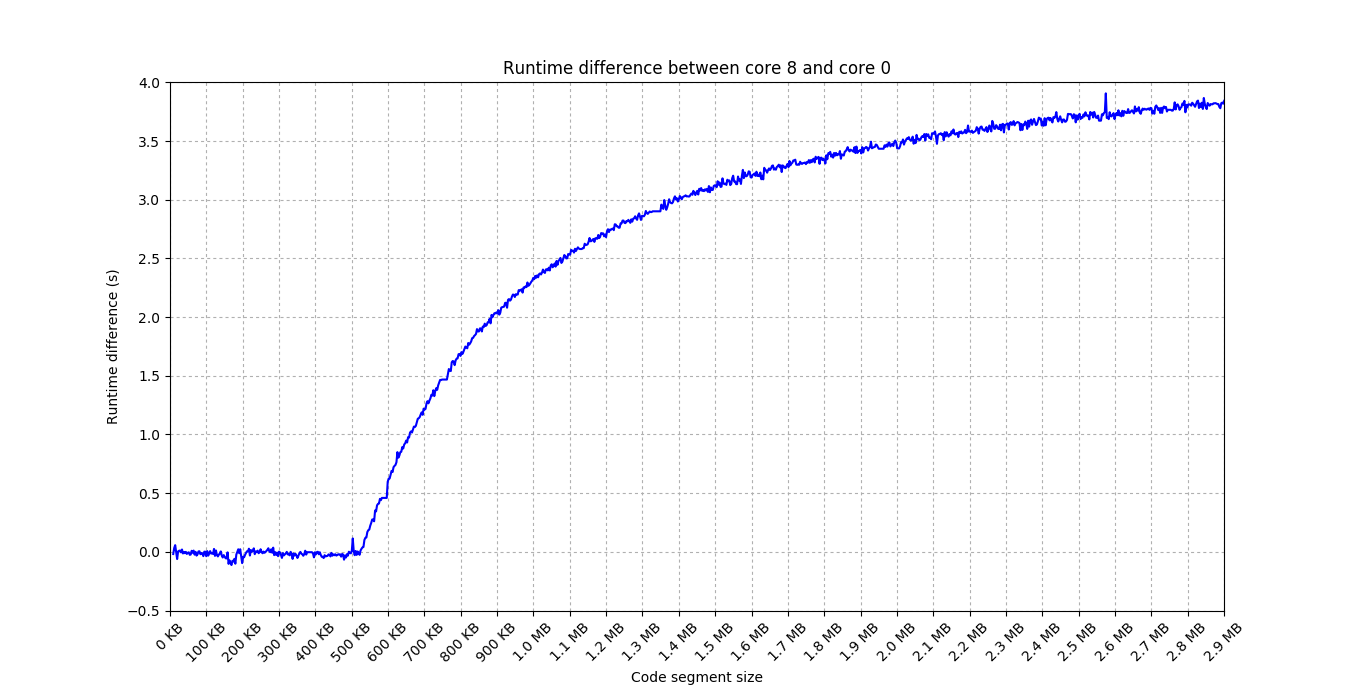
\includegraphics[scale=0.40]{images/runtime_difference.png}
%\end{center}
%\caption{\label{fig:runtime-difference} Runtime difference between core 8 and core 0.}
%\end{figure}

\pgfplotsset{xlabel style={font=\scriptsize},
             ylabel style={font=\scriptsize},
             yticklabel style={font=\tiny},
             scaled x ticks = false,
             xticklabel style={font=\tiny,rotate=0},
             legend style={at={(0.98,0.2)}, font=\sffamily\tiny},
             grid style={dash pattern = on 0.1mm off 0.5mm,gray}
}
\pgfplotstableread{runtime_difference.data}{\pistonkinetics}
\begin{figure}
\begin{center}
\caption{Runtime difference between core 8 and core 0}
\begin{tikzpicture}[scale=1.5]
\label{fig:runtime-difference}
\begin{axis}[xtick={0, 524288, 1048576, 2915678},
             xticklabels={0, 512KiB, 1 MiB, 2.8 MiB },
             grid=both,minor tick num=1,
             ylabel=Runtime difference (s),
             xlabel= Code segment size (bytes),
              legend entries={Runtime difference (Core 8 - Core 0)}]

\addplot [blue, thin] table [x={code}, y={difference}] {\pistonkinetics};


\end{axis}
\end{tikzpicture}
\end{center}
\end{figure}

\section{Conclusions}
When running specific workloads on dual socket Haswell-EP platforms, we observed a 
difference in performance between the first core of the second CPU and the other 
cores on the system. Synthetic benchmarks written during this study require up to 20\% additional 
time to complete on the first core of the second CPU. This asymmetry has been 
reproduced on Haswell-EP, Haswell-EX and Broadwell-EP platforms. The results of
our deep investigation suggest that lower performance on core 8 be caused
by a different behaviour in handling iTLB misses: as a consequence, different
runtime can be observed only with workloads that generate a high number of
such events. At this stage we are unable to provide a conclusive explanation for
this asymmetry.

%\section{Hypothesis disproved so far}
%The following hypothesis have been taken into account so far, without however
%leading to a satisfactory explanation:

%\begin{itemize}
%\item \textit{ksoftirq is using more clock cycles on core 8, therefore there
%appears to be more interrupt activity (at least top half) on this specific core.}
%\\
%The additional number of cycles spent in \textit{\_\_do\_softirq} does not justify
%the slowdown observed. The profiles of the benchmark described in section
%\ref{section:benchmark-itlb} with $n = 32000$ show that \textit{\_\_do\_softirq}
%and \textit{do\_softirq} are responsible respectively for 0.08\% and 0.05\% of the
%additional clock cycles on core 8. The higher number of cycles spent in softirq
%seems to be a consequence rather than a cause. In the Linux kernel the top half
%of the timer interrupt is implemented with a softirq, so it makes sense to have
%a higher number softirqs running if the runtime of the benchmark is itself longer
%(1ms jiffie).
%\end{itemize}

\newpage
\newpage
\begin{appendices}
\label{appendix:function-recordings}
\section{Function annotations}
\begin{minipage}{\linewidth}
\begin{lstlisting}[language={[x64]Assembler}, basicstyle=\ttfamily\tiny,
caption=G4StepLimiter::PostStepGetPhysicalInteractionLength cycles annotation]
Percent |      Source code & Disassembly of libG4processes.so for  cycles:pp
-----------------------------------------------------------------------------
         :      Disassembly of section .text:
         :
         :      000000000032fab0 <G4StepLimiter::PostStepGetPhysicalInteractionLength(G4Track const&, double, G4ForceCondition*)>:
         :      _ZN13G4StepLimiter36PostStepGetPhysicalInteractionLengthERK7G4TrackdP16G4ForceCondition():
   39.78 :        32fab0:       push   %rbx
    0.12 :        32fab1:       movl   $0x2,(%rdx)
         :      _ZNK7G4Track9GetVolumeEv():
    0.00 :        32fab7:       xor    %eax,%eax
         :      _ZNK24G4ReferenceCountedHandleI12G4VTouchableEcvbEv():
    0.73 :        32fab9:       mov    0x40(%rsi),%rdx
         :      _ZN13G4StepLimiter36PostStepGetPhysicalInteractionLengthERK7G4TrackdP16G4ForceCondition():
    0.24 :        32fabd:       mov    %rsi,%rbx
         :      _ZNK7G4Track9GetVolumeEv():
    2.57 :        32fac0:       test   %rdx,%rdx
    0.00 :        32fac3:       je     32fad1 <G4StepLimiter::PostStepGetPhysicalInteractionLength(G4Track const&, double, ...)+0x21>
         :      _ZNK24G4ReferenceCountedHandleI12G4VTouchableEptEv():
    5.88 :        32fac5:       mov    0x8(%rdx),%rdi
         :      _ZNK7G4Track9GetVolumeEv():
    0.24 :        32fac9:       xor    %esi,%esi
    7.47 :        32facb:       mov    (%rdi),%rax
    4.04 :        32face:       callq  *0x20(%rax)
    9.06 :        32fad1:       mov    0x28(%rax),%rax
   10.04 :        32fad5:       mov    0x40(%rax),%rdi
         :      _ZNK15G4LogicalVolume13GetUserLimitsEv():
    0.00 :        32fad9:       test   %rdi,%rdi
    0.61 :        32fadc:       je     32faf8 <G4StepLimiter::PostStepGetPhysicalInteractionLength(G4Track const&, double, ...)+0x48>
    [...]
\end{lstlisting}
\end{minipage}

\begin{minipage}{\linewidth}
\begin{lstlisting}[language={[x64]Assembler},basicstyle=\ttfamily\tiny,
caption=\_\_sin\_avx cycles annotation]
Percent |      Source code & Disassembly of libm-2.17.so for  cycles:pp
------------------------------------------------------------------------
         :      Disassembly of section .text:
         :
         :      0000000000064a30 <__sin_avx>:
         :      __sin_avx():
    6.73 :        64a30:       push   %r12
   24.77 :        64a32:       vmovapd %xmm0,%xmm2
    4.10 :        64a36:       push   %rbp
    1.23 :        64a37:       push   %rbx
    0.00 :        64a38:       sub    $0x70,%rsp
    0.70 :        64a3c:       vstmxcsr 0x50(%rsp)
    2.01 :        64a42:       mov    0x50(%rsp),%ebx
    0.00 :        64a46:       mov    %ebx,%eax
    0.67 :        64a48:       and    $0x9f,%ah
    0.59 :        64a4b:       cmp    %eax,%ebx
    0.00 :        64a4d:       mov    %eax,0x60(%rsp)
    0.32 :        64a51:       jne    6682b <__sin_avx+0x1dfb>
    0.00 :        64a57:       xor    %ebp,%ebp
    0.00 :        64a59:       vmovsd %xmm2,(%rsp)
    0.03 :        64a5e:       mov    (%rsp),%rdx
    [...]
\end{lstlisting}
\end{minipage}

\begin{minipage}{\linewidth}
\begin{lstlisting}[language={[x64]Assembler}, basicstyle=\ttfamily\tiny,
caption=G4VEnergyLossProcess::PostStepGetPhysicalInteractionLength cycles annotation]
Percent |      Source code & Disassembly of libG4processes.so for  cycles:pp
-----------------------------------------------------------------------------
         :      Disassembly of section .text:
         :
         :      00000000003c77b0 <G4VEnergyLossProcess::PostStepGetPhysicalInteractionLength(G4Track const&, double, G4ForceCondition*)>:
         :      _ZN20G4VEnergyLossProcess36PostStepGetPhysicalInteractionLengthERK7G4TrackdP16G4ForceCondition():
   15.07 :        3c77b0:       push   %r14
    0.00 :        3c77b2:       movapd %xmm0,%xmm3
    0.17 :        3c77b6:       push   %r13
    0.11 :        3c77b8:       push   %r12
    0.28 :        3c77ba:       push   %rbp
    0.00 :        3c77bb:       push   %rbx
    0.11 :        3c77bc:       mov    %rdi,%rbx
    0.50 :        3c77bf:       sub    $0x50,%rsp
         :      _ZNK7G4Track21GetMaterialCutsCoupleEv():
    0.17 :        3c77c3:       mov    0x78(%rsi),%rax
         :      _ZN20G4VEnergyLossProcess36PostStepGetPhysicalInteractionLengthERK7G4TrackdP16G4ForceCondition():
    0.06 :        3c77c7:       movl   $0x2,(%rdx)
         :      _ZNK7G4Track21GetMaterialCutsCoupleEv():
    0.94 :        3c77cd:       mov    0x10(%rax),%rax
    1.32 :        3c77d1:       mov    0x68(%rax),%rax
         :      _ZN20G4VEnergyLossProcess14DefineMaterialEPK20G4MaterialCutsCouple():
    0.50 :        3c77d5:       cmp    0x3c0(%rdi),%rax
    1.16 :        3c77dc:       je     3c780c <G4VEnergyLossProcess::PostStepGetPhysicalInteractionLength(...)+0x5c>
    1.82 :        3c77de:       mov    0x10(%rax),%rdx
    [...]
\end{lstlisting}
\end{minipage}

\begin{minipage}{\linewidth}
\begin{lstlisting}[language={[x64]Assembler}, basicstyle=\ttfamily\tiny,
caption=FADS::FadsSteppingAction::UserSteppingAction cycles annotation]
Percent |      Source code & Disassembly of libFadsActions.so for  cycles:pp
-----------------------------------------------------------------------------
         :      Disassembly of section .text:
         :
         :      00000000000087f0 <FADS::FadsSteppingAction::UserSteppingAction(G4Step const*)>:
         :      _ZN4FADS18FadsSteppingAction18UserSteppingActionEPK6G4Step():
   28.47 :        87f0:       push   %r12
    0.00 :        87f2:       push   %rbp
    0.10 :        87f3:       mov    %rdi,%rbp
    0.10 :        87f6:       push   %rbx
    0.19 :        87f7:       mov    %rsi,%rbx
    0.00 :        87fa:       sub    $0x20,%rsp
    8.30 :        87fe:       cmpb   $0x0,0x8fa3(%rip)
    0.58 :        8805:       je     8900 <FADS::FadsSteppingAction::UserSteppingAction(G4Step const*)+0x110>
    2.99 :        880b:       cmpb   $0x0,0x8d8e(%rip)    # 115a0 <FADS::FadsSteppingAction::UserSteppingAction(G4Step const*)::first>
    0.97 :        8812:       jne    8960 <FADS::FadsSteppingAction::UserSteppingAction(G4Step const*)+0x170>
    0.68 :        8818:       mov    0x8f91(%rip),%rax    # 117b0 <FADS::FadsSteppingAction::UserSteppingAction(G4Step const*)::act>
   11.87 :        881f:       mov    -0x18(%rax),%rsi
    0.00 :        8823:       test   %rsi,%rsi
    0.87 :        8826:       je     88a5 <FADS::FadsSteppingAction::UserSteppingAction(G4Step const*)+0xb5>
    0.00 :        8828:       mov    0x8891(%rip),%r12    # 110c0 <_DYNAMIC+0x388>
    [...]
\end{lstlisting}
\end{minipage}

\begin{minipage}{\linewidth}
\begin{lstlisting}[language={[x64]Assembler}, basicstyle=\ttfamily\tiny,
caption=G4CrossSectionDataStore::GetCrossSection cycles annotation]
Percent |      Source code & Disassembly of libG4processes.so for  cycles:pp
-----------------------------------------------------------------------------
         :      Disassembly of section .text:
         :
         :      00000000005bbc00 <G4CrossSectionDataStore::GetCrossSection(G4DynamicParticle const*, G4Element const*, double)>:
         :      _ZN23G4CrossSectionDataStore15GetCrossSectionEPK17G4DynamicParticlePK9G4Elementd():
   14.85 :        5bbc00:       push   %r15
    0.17 :        5bbc02:       push   %r14
    1.26 :        5bbc04:       push   %r13
    1.76 :        5bbc06:       mov    %rdx,%r13
    0.25 :        5bbc09:       push   %r12
    0.00 :        5bbc0b:       mov    %rsi,%r12
    1.17 :        5bbc0e:       push   %rbp
    0.84 :        5bbc0f:       mov    %rdi,%rbp
    0.84 :        5bbc12:       push   %rbx
    1.01 :        5bbc13:       sub    $0x58,%rsp
    5.87 :        5bbc17:       mov    0x18(%rdi),%eax
    0.00 :        5bbc1a:       movsd  %xmm0,0x8(%rsp)
    0.25 :        5bbc20:       test   %eax,%eax
    0.00 :        5bbc22:       je     5bbf6c <G4CrossSectionDataStore::GetCrossSection(...)+0x59>
    0.84 :        5bbc28:       sub    $0x1,%eax
    [...]
\end{lstlisting}
\end{minipage}

\begin{minipage}{\linewidth}
\begin{lstlisting}[language={[x64]Assembler}, basicstyle=\ttfamily\tiny,
caption=G4FieldTrack::G4FieldTrack cycles annotation]
 Percent |      Source code & Disassembly of libG4geometry.so for  cycles:pp
----------------------------------------------------------------------------
         :      Disassembly of section .text:
         :
         :      00000000000bc9c0 <G4FieldTrack::G4FieldTrack(...)>:
         :      _ZN12G4FieldTrackC2ERKN5CLHEP10Hep3VectorES3_ddddddPS2_():
    7.76 :        bc9c0:       sub    $0x88,%rsp
    0.13 :        bc9c7:       movsd  %xmm2,0x40(%rdi)
    0.92 :        bc9cc:       addsd  %xmm2,%xmm2
    0.39 :        bc9d0:       movsd  %xmm4,0x48(%rdi)
    0.00 :        bc9d5:       movabs $0x7fefffffffffffff,%rax
    0.26 :        bc9df:       movq   $0x0,0x58(%rdi)
    0.66 :        bc9e7:       movapd %xmm0,%xmm3
    1.18 :        bc9eb:       movsd  %xmm1,0x38(%rdi)
    0.00 :        bc9f0:       movsd  %xmm5,0x50(%rdi)
    0.00 :        bc9f5:       movq   $0x0,0x60(%rdi)
    1.58 :        bc9fd:       addsd  %xmm1,%xmm2
    0.26 :        bca01:       movq   $0x0,0x68(%rdi)
    0.53 :        bca09:       movq   $0x0,0x70(%rdi)
    0.13 :        bca11:       movq   $0x0,0x78(%rdi)
    1.18 :        bca19:       movq   $0x0,0x80(%rdi)
\end{lstlisting}
\end{minipage}

\begin{minipage}{\linewidth}
\begin{lstlisting}[language={[x64]Assembler}, basicstyle=\ttfamily\tiny,
caption=\_\_log10\_finite cycles annotation, label=lst:log10]
Percent |      Source code & Disassembly of libm-2.17.so for  cycles:pp
------------------------------------------------------------------------
         :      Disassembly of section .text:
         :
         :      0000000000014690 <__log10_finite>:
         :      __ieee754_log10():
    7.59 :        14690:       movabs $0xfffffffffffff,%rcx
    0.00 :        1469a:       movq   %xmm0,%rax
    0.00 :        1469f:       cmp    %rcx,%rax
    1.60 :        146a2:       jg     146d8 <__log10_finite+0x48>
    0.00 :        146a4:       movabs $0x7fffffffffffffff,%rdx
    0.00 :        146ae:       test   %rdx,%rax
    0.00 :        146b1:       je     14770 <__log10_finite+0xe0>
    0.00 :        146b7:       test   %rax,%rax
    0.00 :        146ba:       js     1478f <__log10_finite+0xff>
    0.00 :        146c0:       mulsd  0x74b18(%rip),%xmm0        # 891e0 <sqrt_2.2977+0x10>
    0.00 :        146c8:       mov    $0xfffffbcb,%ecx
    0.00 :        146cd:       movq   %xmm0,%rdx
    0.00 :        146d2:       jmp    146e0 <__log10_finite+0x50>
    0.00 :        146d4:       nopl   0x0(%rax)
    0.27 :        146d8:       mov    %rax,%rdx
\end{lstlisting}
\end{minipage}


\end{appendices}
\section*{References}
\bibliography{iopart-num}
\bibliographystyle{unsrt}
\end{document}
